
%(BEGIN_QUESTION)
% Copyright 2006, Tony R. Kuphaldt, released under the Creative Commons Attribution License (v 1.0)
% This means you may do almost anything with this work of mine, so long as you give me proper credit

Calculate the net torque applied to the drum from the two forces shown.  The drum's outside radius is 6 feet, and the radius of the smaller pulley (attached to the drum) is 2 feet:

$$\includegraphics[width=15.5cm]{i01428x01.eps}$$

Also, calculate the mechanical advantage of this system, if $F_1$ is considered the {\it input} force.

\underbar{file i01428}
%(END_QUESTION)





%(BEGIN_ANSWER)

$\tau_{net}$ = 11.2 lb-ft, clockwise
 
\vskip 10pt

$$M_A = {F_{out} \over F_{in}} = {3.2 \hbox{ lb} \over 4 \hbox{ lb}} = 0.8$$

%(END_ANSWER)





%(BEGIN_NOTES)

%INDEX% Machine, mechanical advantage
%INDEX% Physics, torque: calculation problem

%(END_NOTES)


